% ============================================================
%  SCHOLA DOMESTICA — Magister Mathematica
%  Level 1 | Week 6 | Day 1
%  Topic: Numbers 0–10 — Mixed Review & the Number Line
%  Enrichment: Mayan Dot-Bar Counting (1–5)
% ============================================================
\documentclass[12pt, letterpaper]{article}

\usepackage[top=1in, bottom=1in, left=1in, right=1in]{geometry}
\usepackage{fontenc}
\usepackage{inputenc}
\usepackage{lmodern}
\usepackage{microtype}
\usepackage{amsmath}
\usepackage{graphicx}
\usepackage{xcolor}
\usepackage{tikz}
\usepackage{array}
\usepackage{enumitem}
\usepackage{multicol}
\usepackage{mdframed}
\usepackage{fancyhdr}

\definecolor{scholared}{RGB}{160,30,30}
\definecolor{scholagold}{RGB}{180,140,40}
\definecolor{scholacream}{RGB}{253,248,235}
\definecolor{scholagreen}{RGB}{50,110,60}
\definecolor{scholablue}{RGB}{40,80,140}
\definecolor{mayared}{RGB}{140,30,30}

\pagestyle{fancy}
\fancyhf{}
\renewcommand{\headrulewidth}{0.6pt}
\fancyhead[L]{\small\textcolor{scholared}{\textbf{Schola Domestica — Magister Mathematica}}}
\fancyhead[R]{\small\textcolor{scholared}{Level 1 · Week 6 · Day 1}}
\fancyfoot[C]{\small\textcolor{gray}{— \thepage\ —}}

\newcommand{\answerline}{\underline{\hspace{2.5cm}}}
\newcommand{\biganswerline}{\underline{\hspace{4cm}}}
\newcommand{\numbox}{\fbox{\hspace{0.6cm}\vphantom{0}}}
\newcommand{\symbox}{\fbox{\hspace{0.7cm}}}

\newmdenv[
  backgroundcolor=scholacream,
  linecolor=scholared,
  linewidth=1.5pt,
  roundcorner=6pt,
  innertopmargin=8pt,
  innerbottommargin=8pt,
  innerleftmargin=10pt,
  innerrightmargin=10pt
]{lessonbox}

\newmdenv[
  backgroundcolor={RGB}{240,235,210},
  linecolor=mayared,
  linewidth=1.5pt,
  roundcorner=6pt,
  innertopmargin=8pt,
  innerbottommargin=8pt,
  innerleftmargin=10pt,
  innerrightmargin=10pt
]{mayanbox}

% Mayan glyph: n dots (row) above a bar or bars
% We draw it manually in TikZ
\newcommand{\mayanone}{%

\begin{tikzpicture}[baseline=0.2ex,scale=0.7]
  \filldraw[mayared] (0.25,0.5) circle (0.18cm);
\end{tikzpicture}}

\newcommand{\mayantwo}{%

\begin{tikzpicture}[baseline=0.2ex,scale=0.7]
  \filldraw[mayared] (0.1,0.5) circle (0.18cm);
  \filldraw[mayared] (0.55,0.5) circle (0.18cm);
\end{tikzpicture}}

\newcommand{\mayanthree}{%

\begin{tikzpicture}[baseline=0.2ex,scale=0.7]
  \foreach \i in {1,2,3}{\filldraw[mayared](\i*0.35-0.1,0.5)circle(0.18cm);}
\end{tikzpicture}}

\newcommand{\mayanfour}{%

\begin{tikzpicture}[baseline=0.2ex,scale=0.7]
  \foreach \i in {1,...,4}{\filldraw[mayared](\i*0.35-0.1,0.5)circle(0.18cm);}
\end{tikzpicture}}

\newcommand{\mayanfive}{%

\begin{tikzpicture}[baseline=0.2ex,scale=0.7]
  \draw[mayared, line width=2.5pt] (0,0) -- (1.2,0);
\end{tikzpicture}}

\begin{document}

\begin{center}
  {\LARGE\textbf{\textcolor{scholared}{Numbers 0–10: Mixed Review}}}\\[4pt]
  {\Large\textcolor{scholagold}{\textit{Counting, Comparing, and the Number Line}}}\\[6pt]
  {\small Name: \biganswerline \hspace{1cm} Date: \answerline}
\end{center}

\vspace{4pt}
\noindent\textcolor{scholared}{\rule{\linewidth}{1pt}}
\vspace{4pt}

% IMAGE PROMPT (Miyazaki-style watercolour):
% A countryside path winding through a green field with wildflowers. Along the path are 11
% small stone markers numbered 0 to 10, each half-hidden by grass. A child in a straw hat
% walks between marker 6 and marker 7. Soft watercolour, warm afternoon light.
% No text visible on markers in the actual image.

\begin{lessonbox}
\textbf{What we know about numbers 0–10:}
\begin{itemize}[leftmargin=1.5em, itemsep=2pt]
  \item They live in order on the \textbf{number line}: $0, 1, 2, 3, 4, 5, 6, 7, 8, 9, 10$
  \item We can compare them: $<$ (less than), $>$ (greater than), $=$ (equal to)
  \item \textbf{0} means \textit{nothing}. \textbf{10} is the greatest number we know so far.
\end{itemize}
\end{lessonbox}

\bigskip

% ===== PART I: NUMBER LINE HOPS =====
\noindent\textcolor{scholared}{\large\textbf{Part I — Number Line Hops}} \hfill \textit{(Problems 1–6)}

\medskip

\begin{center}
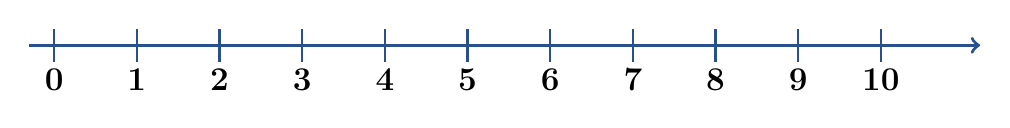
\begin{tikzpicture}[scale=1.05]
  \draw[very thick, scholablue, ->] (-0.3,0) -- (11.2,0);
  \foreach \n in {0,...,10} {
    \draw[thick, scholablue] (\n,0.2) -- (\n,-0.2);
    \node[below=5pt] at (\n,0) {\large\textbf{\n}};
  }
\end{tikzpicture}
\end{center}

\medskip
\noindent\textit{Use the number line above to answer each question.}

\bigskip
\begin{multicols}{2}
\noindent\textbf{1.} Hop 1 forward from 6: \hfill \answerline \\[12pt]
\noindent\textbf{2.} Hop 2 forward from 7: \hfill \answerline \\[12pt]
\noindent\textbf{3.} Hop 1 backward from 9: \hfill \answerline

\columnbreak

\noindent\textbf{4.} Hop 2 backward from 10: \hfill \answerline \\[12pt]
\noindent\textbf{5.} Start at 6, hop to 10. How many hops? \hfill \answerline \\[12pt]
\noindent\textbf{6.} Start at 10, hop back to 7. How many hops? \hfill \answerline
\end{multicols}

\bigskip
\noindent\textcolor{scholared}{\rule{\linewidth}{0.4pt}}

% ===== PART II: MIXED COMPARE =====
\noindent\textcolor{scholared}{\large\textbf{Part II — Compare with $<$, $>$, $=$}} \hfill \textit{(Problems 7–12)}

\bigskip
\begin{multicols}{3}
\noindent\textbf{7.} $6$ \; \symbox \; $10$ \\[14pt]
\noindent\textbf{8.} $9$ \; \symbox \; $7$ \\

\columnbreak
\noindent\textbf{9.} $8$ \; \symbox \; $8$ \\[14pt]
\noindent\textbf{10.} $0$ \; \symbox \; $1$ \\

\columnbreak
\noindent\textbf{11.} $10$ \; \symbox \; $6$ \\[14pt]
\noindent\textbf{12.} $7$ \; \symbox \; $9$
\end{multicols}

\bigskip
\noindent\textcolor{scholared}{\rule{\linewidth}{0.4pt}}

% ===== PART III: FILL THE SEQUENCE =====
\noindent\textcolor{scholared}{\large\textbf{Part III — Fill the Missing Numbers}} \hfill \textit{(Problems 13–14)}

\bigskip
\noindent\textbf{13.} Count forward — fill the boxes:

\medskip
\hspace{2em} 5 \; , \; \numbox \; , \; \numbox \; , \; 8 \; , \; \numbox \; , \; 10

\bigskip
\noindent\textbf{14.} Count backward — fill the boxes:

\medskip
\hspace{2em} 10 \; , \; \numbox \; , \; 8 \; , \; \numbox \; , \; 6 \; , \; \numbox

\bigskip
\noindent\textcolor{scholared}{\rule{\linewidth}{0.4pt}}

% ===== ENRICHMENT =====
\begin{mayanbox}
\textcolor{mayared}{\textbf{Enrichment — The Mayan Way to Count}}\\[6pt]
\noindent Long ago, the Maya people of Mexico and Central America used \textbf{dots and bars} to write numbers.\\[4pt]
A \textbf{dot} $(\bullet)$ means \textbf{1}. \quad A \textbf{bar} $(\rule{1cm}{2pt})$ means \textbf{5}.\\[8pt]
\begin{center}
\renewcommand{\arraystretch}{1.6}
\begin{tabular}{|c|c|c|c|c|}
\hline
\mayanone & \mayantwo & \mayanthree & \mayanfour & \mayanfive \\
\hline
\textbf{1} & \textbf{2} & \textbf{3} & \textbf{4} & \textbf{5} \\
\hline
\end{tabular}
\end{center}
\medskip
\noindent\textit{Look at the Mayan glyphs above. What does \mayanfive\ mean?} \quad \answerline\\[6pt]
\noindent\textit{How many dots are in \mayanthree?} \quad \answerline
\end{mayanbox}

\end{document}
